\documentclass[12pt]{article}
\usepackage{times}
\usepackage[hungarian,british]{babel}
\usepackage{url}
\usepackage{latexsym}
\usepackage[utf8]{inputenc}
\usepackage[hidelinks]{hyperref}
\usepackage{color}
\usepackage{graphicx}
\usepackage{booktabs,amsmath,multicol,bm}
\usepackage{breakcites}
\usepackage{float}
\usepackage[nottoc]{tocbibind}
\setcounter{secnumdepth}{3}
\usepackage[top=2.5cm, bottom=4cm, left=2.5cm, right=2.5cm]{geometry}

\begin{document}
	\title{Deep Learning Based Chatbot Models}
	\author{Richárd Krisztián Csáky \\ Budapest University of Technology and Economics}
	\date{\today}
	
\begin{titlepage}
		\centering
		
\includegraphics[width=0.6\textwidth]{pics/bme_logo_nagy.eps}\par\vspace{1cm}
		{\scshape Budapest University of Technology and Economics \\ Faculty of Electrical Engineering and Informatics \\
			Department of Automation and Applied Informatics \par}
		\vspace{2cm}
		{\huge\mdseries Deep Learning Based Chatbot Models\par}
		\vspace{0.5cm}
		{\scshape\Large Scientific Students' Associations Report\par}
		\vspace{1.5cm}
		
		{\Large Author: \\ Richárd Krisztián Csáky\par}
		\vspace{1.5cm}
		{\Large Supervised by \\ Gábor Recski\par}
		\vfill
		\par
		{\Large 2017\par}
		
		
\end{titlepage}

\begin{otherlanguage}{hungarian}
\begin{abstract}
A konverzációs ágens (chatbot) egy olyan program, mely természetes nyelvet használva képes emberekkel kommunikálni. A beszélgetés modellezése fontos feladat a természetes nyelvfeldolgozás és mesterséges intelligencia (MI) területén. Az MI tudományág megszületése óta egy jól működő chatbot létrehozása még mindig az egyik legnehezebb kihívás. A chatbotok sokféle feladatra használhatók, de mindegyik esetében elvárt, hogy megértsék a felhasználó mondandóját és az adott problémához releváns válaszokat generáljanak.
		
A múlt chatbot architektúrái kézi szabályokra és sablonokra, vagy egyszerű statisztikai módszerekre támaszkodtak. 2015 óta, a  mélytanulás (deep learning) elterjedésével ezek a modellek gyorsan felcserélődtek elejétől végéig tanítható neurális hálózatokkal. Manapság a rekurrens enkóder-dekóder modell \cite{Cho:2014} dominál a konverzáció modellezésben. Ezt az architektúrát a neurális gépi fordítás területéről adaptálták, ahol rendkívül jó eredményeket ért el. Azóta sokféle változata \cite{Serban:2015} és kiegészítése született annak érdekében, hogy minél jobb minőségű legyen a chatbotok által folytatott beszélgetés.
		
Munkám során részletes irodalmi kutatást végeztem, melyben az elmúlt 3 évben publikált, több mint 70, a chatbotokkal kapcsolatos publikációt vizsgálok meg. Ezután amellett érvelek, hogy a konverzáció modellezés sajátosságai a jelenlegi state-of-the-art architektúráktól eltérő megközelítést igényelnek. Szakirodalmi példákon alapulva bemutatom, hogy a jelenlegi chatbot modellek miért nem vesznek figyelembe elég ún. priort a válasz generálása során, és ez hogyan befolyásolja a beszélgetés minőségét. Ezek a priorok olyan külső információt hordoznak, melyen a beszélgetés kondicionálva lehet, mint például a beszélők személye \cite{Li:2016} vagy hangulata. Amellett, hogy bemutatom az okait, javaslatokat is teszek a probléma orvoslására.
		
A dolgozat következő részében egy nemrég bemutatott modellt, mely jelenleg state-of-the-art-nak számít a neurális gépi fordításban, az úgynevezett Transformer-t \cite{Vaswani:2017} adaptálom a beszélgetés-modellezés feladatára. Először az eredeti cikkben leírt modell tanításával kísérletezek, tanítóadatként a Cornell Movie-Dialog Corpus \cite{Danescu:2011} dialógusait használva. Emellett továbbfejlesztem a modellt saját, az enkóder-dekóder architektúra hiányainak orvoslására született ötletekkel. További priorokat adok bemenetként a modellbe, mint a beszélgetők személye vagy hangulata. Végül korábbi chatbot modellekkel való összehasonlítás útján részletes elemzést végzek arról, hogy az eredeti modell mennyire teljesít jól dialógus adattal és hogyan befolyásolják a generált válaszok minőségét az általam implementált további kiegészítések.
\end{abstract}
\end{otherlanguage}


\newpage\begin{abstract}
A conversational agent (chatbot) is a piece of software that is able to communicate with humans using natural language. Modelling conversation is an important task in natural language processing and artificial intelligence (AI). Indeed, ever since the birth of AI, creating a good chatbot remains one of the field’s hardest challenges. While chatbots can be used for various tasks, in general they have to understand users’ utterances and provide responses that are relevant to the problem at hand.

In the past, methods for constructing chatbot architectures have relied on hand-written rules and templates or simple statistical methods. With the rise of deep learning these models were quickly replaced by end-to-end trainable neural networks around 2015. More specifically, the recurrent encoder-decoder model \cite{Cho:2014} dominates the task of conversational modelling. This architecture was adapted from the neural machine translation domain, where it performs extremely well. Since then a multitude of variations \cite{Serban:2015} and features were presented that augment the quality of the conversation that chatbots are capable of.

In my work, I conduct an in-depth survey of recent literature, examining over 70 publications related to chatbots published in the last 3 years. Then I proceed to make the argument that the very nature of the general conversation domain demands approaches that are different from current state-of-the-art architectures. Based on several examples from the literature I show why current chatbot models fail to take into account enough priors when generating responses and how this affects the quality of the conversation. In the case of chatbots these priors can be outside sources of information that the conversation is conditioned on like the persona \cite{Li:2016} or mood of the conversers. In addition to presenting the reasons behind this problem, I propose several ideas on how it could be remedied.

The next section of my paper focuses on adapting the very recent Tranformer \cite{Vaswani:2017} model to the chatbot domain, which is currently the state-of-the-art in neural machine translation. I first present my experiments with the vanilla model, using conversations extracted from the Cornell Movie-Dialog Corpus \cite{Danescu:2011}. Secondly, I augment the model with some of my ideas regarding the issues of encoder-decoder architectures. More specifically, I feed additional features into the model like mood or persona together with the raw conversation data. Finally, I conduct a detailed analysis of how the vanilla model performs on conversational data by comparing it to previous chatbot models and how the additional features, affect the quality of the generated responses.
\end{abstract}

\newpage\tableofcontents
\newpage\section{Introduction} \label{sec:intro}

A conversational agent (chatbot) is a piece of software that is able to communicate with humans using natural language. Ever since the birth of AI, modelling conversations remains one of the field's toughest challenges. Even though they are far from perfect, chatbots are now used in a plethora of applications like Apple's Siri \cite{Siri:2017}, Google's Google Assistant \cite{Google:2017} or Microsoft's Cortana \cite{Cortana:2017}. In order to fully understand the capabilities and limitations of current chatbot architectures and techniques I conduct an in-depth survey, where I examine related literature published over the past 3 years and I implement my own chatbot based on a novel neural network model. 

The paper begins with a brief overview of the history of chatbots in Section~\ref{sec:history}, where I discuss the properties and objectives of conversational modelling. I present early approaches and the current dominating model based on neural networks for building conversational agents.

In the following section I present key architectures and techniques that were developed over the past 3 years relating to chatbots. I group publications into 11 groups based on the specific techniques or approaches that are discussed by the authors. After this I present criticism regarding some of the properties of current chatbot models and I show how several of the techniques used are inappropriate for the task of modelling conversations.

In the next section I conduct experiments by training a novel neural network model, the Transformer \cite{Vaswani:2017} using dialog datasets \cite{Danescu:2011,Tiedemann:2009}. I run several trainings using these datasets detailed in Section~\ref{sec:experiments}. I present the results of the different training setups by qualitatively comparing them to previous chatbot models and by using standard evaluation metrics.

In the final section before concluding I offer possible directions for future work. More specifically, I propose several ideas in order to remedy the problems discussed in Section~\ref{ssec:32}.

\newpage\section{History of Chatbots} \label{sec:history}

\subsection{Modelling Conversations} \label{ssec:21}
Chatbot models usually take in as input natural language sentences uttered by the user, and output a response. There are two main approaches for generating responses. The traditional approach is to use hard-coded templates and rules to make chatbots, which I present in Section~\ref{ssec:22}. The more novel approach, which I discuss in detail in Section~\ref{ssec:23} was made possible by the rise of deep learning. Neural network models are trained on large amounts of data to learn the process of generating relevant and grammatically correct responses to input utterances. Models have also been developed to accommodate for spoken or visual inputs. They oftentimes make use of a speech recognition component to transform speech into text \cite{Serban:2017} or convolutional neural networks that transform the input pictures into useful representations for the chatbot \cite{Havrylov:2017}. The latter models are also called visual dialog agents, where the conversation is grounded on both textual and visual input \cite{Das:2017}.

Conversational agents exist in two main forms. The first one is the more traditional task-oriented dialog system, which is limited in its conversational capabilities, however it is very robust at executing task specific commands and requirements. Task-oriented models are built to accomplish a specific task like making restaurant reservations \cite{Joshi:2017,Bordes:2016} or promoting movies \cite{Yu:2017}, just to name a few. These systems often don't have the ability to respond to arbitrary utterances since they are limited to a specific domain, thus users have to be guided by the dialog system towards the task at hand. Usually they are deployed to tasks where some information has to be retrieved from a knowledge base. They are mainly used to replace the process of navigating through menus and user interfaces like making the process of booking flight tickets or finding a public transportation route between two locations conversational \cite{Zhao:2017}.  

The second type of dialog agents are the non-task or open-domain chatbots. These conversation systems try to imitate human dialog in all its facets. This means that one should hardly be able to distinguish such a chatbot from a real human, but current models are still far away from such claims. These models are usually trained with conversation examples extracted from movie scripts or from Twitter-like post-reply pairs \cite{Vinyals:2015,Shang:2015,Serban:2015,Li:2016}. For these models there isn't a well defined goal, but they are required to have a certain amount of world knowledge and commonsense in order to hold conversations about basically anything.

Recently an emphasis has been put on integrating the two types of conversational agents. The main idea is to combine the positive aspects of both types, like the robust abilities of goal-oriented dialog systems to perform tasks and the human-like chattyness of open-domain chatbots \cite{Zhao:2017,Yu:2017,Serban:2017}. This is beneficial because the user is more likely to engage with a task-oriented dialog agent if its more human-like, and handles out of domain responses well.

\subsection{Early Approaches} \label{ssec:22}

ELIZA is one of the first ever chatbot programs written \cite{Weizenbaum:1966}. It uses clever hand-written templates to generate a reply that resembles the user's input utterance. Since then countless hand-coded rule-based chatbots have been written \cite{Wallace:2009,Cleverbot:2017,Mitsuku:2017}. Furthermore, a number of programming frameworks specifically designed to facilitate building dialog agents have been developed \cite{Marietto:2013,Microsoft:2017}.

These chatbot programs are very similar in their core, namely that they all use hand-written rules to generate replies. Usually simple pattern matching or keyword retrieval techniques are employed to handle the user's input utterance. Then rules are used to transform a matching pattern or a keyword into a predefined reply.

\begin{figure}[H]
	\label{fig:22}
	\centering
	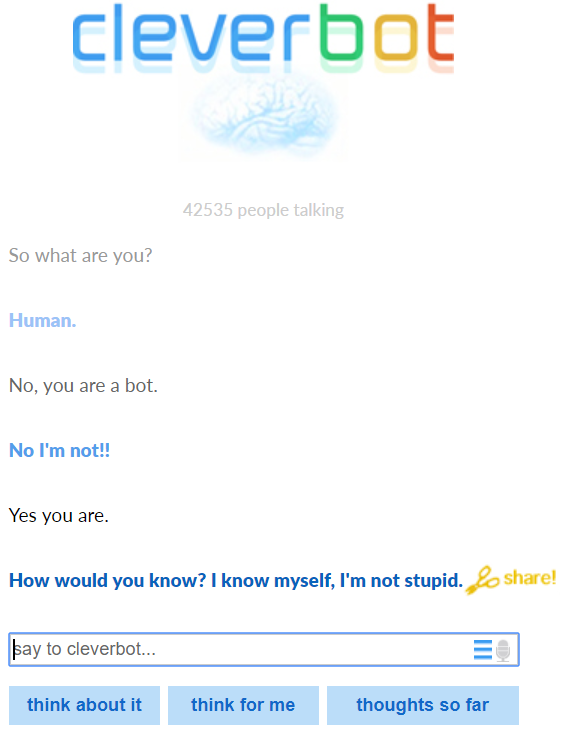
\includegraphics[width=0.4\textwidth]{pics/cleverbot.png}
	\caption{Sample conversation with Cleverbot \cite{Cleverbot:2017}}
\end{figure}

\subsection{The Encoder-Decoder Model} \label{ssec:23}
The main concept that differentiates rule-based and neural network based approaches is the presence of a learning algorithm in the latter case. Instead of using hand-written rules deep learning models transform input sentences into replies directly by using matrix multiplications and non-linearities over millions of parameters. We can further divide neural network based models into two categories, retrieval-based and generative models. The former simply returns a reply from the dataset by computing the most likely response to the current input utterance based on a scoring function, which can be implemented as a neural network \cite{Cho:2014} or by simply computing the cosine similarity between the input utterance and candidate replies \cite{stalemate:2016}. Generative models on the other hand synthesize the reply one word at a time by computing probabilities over the whole vocabulary \cite{Sutskever:2014,Vinyals:2015}. There have also been approaches that integrate the two types of dialog systems by comparing a generated reply with a retrieved reply and determining which one is more likely to be a better response \cite{Song:2016}.

As with many other applications the field of conversational modelling has been transformed by the rise of deep learning. More specifically the encoder-decoder recurrent neural network (RNN) model (also called seq2seq \cite{Sutskever:2014}) introduced by \cite{Cho:2014} and its variations have been dominating the field. This model was originally developed for neural machine translation (NMT), but it was found to be suitable to \textit{translate} source utterances into responses within a conversational setting \cite{Shang:2015,Vinyals:2015}.

\subsubsection{Recurrent Neural Networks} \label{sssec:231}
A recurrent neural network (RNN) \cite{RNN:1988} is a neural network that can take as inputs a variable length sequence \(\bm{x}=(x_1,...,x_n)\), by unfolding itself over each input \(x_i\) and generating a hidden state at each step \(\bm{h}=(\bm{h_1},...,\bm{h_n})\). At each step \(i\), the hidden state \(\bm{h}_i\) is updated by
\begin{equation} \label{eq231a}
\bm{h}_i=f(\bm{h}_{i-1},x_i)
\end{equation}
which is also called the unrolling of the network. \(f\) here is a non-linear activation function. Usually long short-term memory (LSTM) or gated recurrent units (GRU) are used for the activation function \cite{Hochreiter:1997,Cho:2014}. An important characteristic of recurrent neural networks is that the parameters of the function \(f\) don't change during the unrolling of the network.

\begin{figure}[H]
	\label{fig:231}
	\centering
	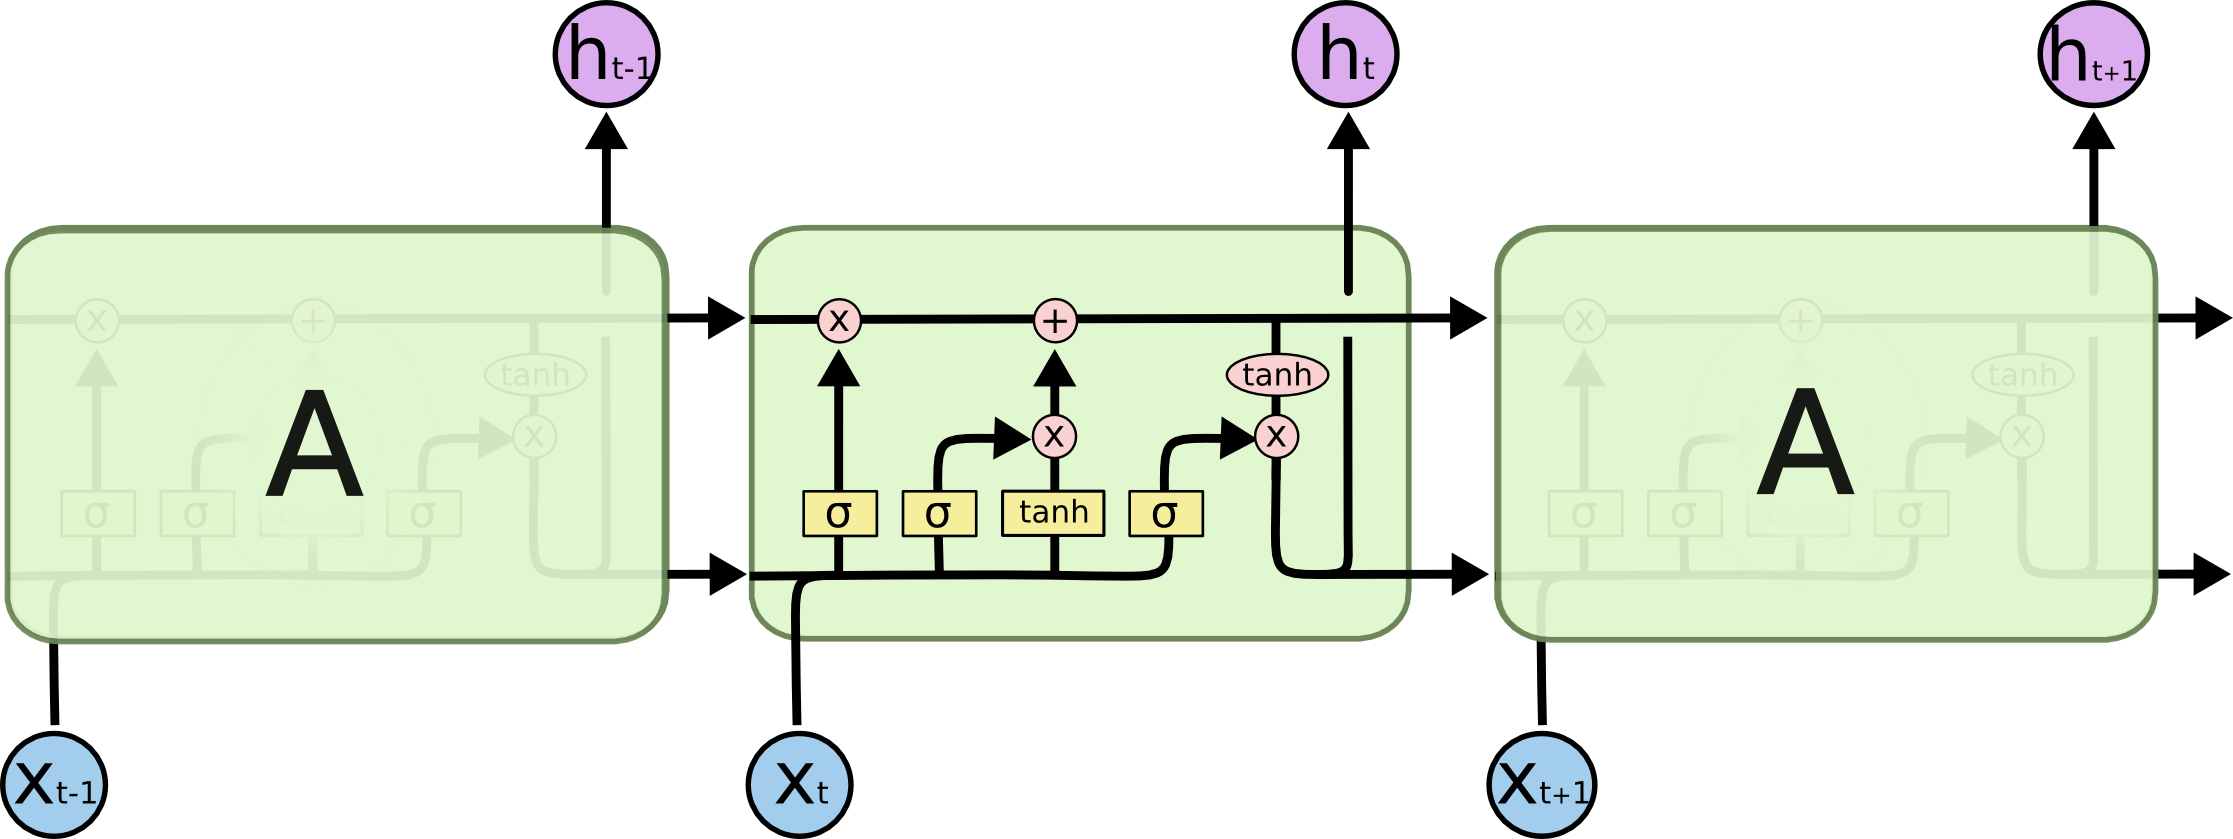
\includegraphics[width=0.7\textwidth]{pics/LSTM.png}
	\caption{Unrolling the LSTM network over 3 time steps \cite{LSTM_pic:2017}}
\end{figure}

RNNs can be used for language modelling by training it to learn the probability distribution over the vocabulary \(\bm{V}\) given an input sequence of words. We can generate this probability distribution to predict the next word in the sequence by taking the hidden state of the RNN in the last step, and feeding it into a softmax activation function
\begin{equation} \label{eq231b}
p(x_{i,j}|x_{i-1},...,x_1)=\frac{exp(\bm{w}_j\bm{h}_i)}{\sum_{j^{'}=1}^{K}exp(\bm{w}_{j^{'}}\bm{h}_i)}
\end{equation}
for all possible words (symbols) \(j=1,...,K\), where \(\bm{w}_j\) are the rows in the weight matrix of the softmax function.

Training of these networks is done via the generalized backpropagation algorithm called truncated backpropagation through time \cite{Werbos:1990,RNN:1988}. Essentially we backpropagate the error through each time step of the network to learn its parameters. The error can be computed by using the cross-entropy loss, which calculates how different the predictions are compared to the true labels.
\begin{equation} \label{eq231c}
L(\bm{y}_i,\bm{\hat{y}}_{i})=-\bm{y}_i log(\bm{\hat{y}}_{i})
\end{equation}
where \(\bm{\hat{y}}_{i}\) is the vector of the predicted probabilities over all words in the vocabulary at step \(i\), and \(\bm{y}_i\) is the one-hot vector over the vocabulary. A one-hot vector is made up of zeros except at the index of the one true word that follows in the sequence, where it is equal to 1. After computing the derivative with respect to all of the weights in the network using the backpropagation through time algorithm we can update the weights in order to get closer to an optimum with optimization techniques like stochastic gradient descent (SGD) \cite{SGD:2010}. 

\subsubsection{The Seq2seq Model}
The sequence to sequence model (seq2seq) was first introduced by \cite{Cho:2014}, but they only used it to re-rank sentences instead of generating completely new ones, which was first done by \cite{Sutskever:2014}. Since then, besides NMT and conversational models a plethora of different applications of these models have been introduced like text summarization \cite{Nallapati:2016}, speech recognition \cite{Chiu:2017}, code generation \cite{Rico:2017} and parsing \cite{Konstas:2017}, just to name a few.

\begin{figure}[H]
	\label{fig:232a}
	\centering
	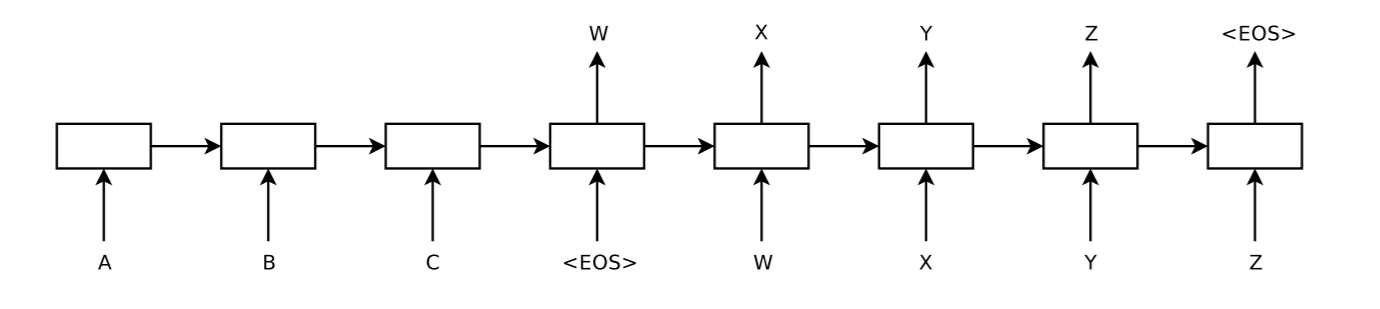
\includegraphics[width=0.9\textwidth]{pics/seq2seq.png}
	\caption{LSTM based Seq2seq model applied to conversational modelling \cite{seq2seq_pic:2017}}
\end{figure}

The simplest and initial form of the model is based on two RNNs. The actual implementation of RNNs can be in the form of LSTMs or GRUs as discussed in Section~\ref{sssec:231}. The goal is two estimate the conditional probability of \(p(y_1,...,y_{N^{'}}|x_1,...,x_N)\), where \(x_1,...,x_N\) is the input sequence and \(y_1,...,y_{N^{'}}\) is the corresponding output sequence. Since two different RNNs are used for the input and output sequences, the length of the sequences, \(N\) and \(N^{'}\) can be different. The encoder RNN is unrolled over the words in the source sequence and its last hidden state is called the thought vector, which is a representation of the whole source sequence. The initial hidden state of the decoder RNN is then set to this representation, and the generation of target sequence words is done by taking the output of the unrolled decoder network at each time-step and feeding it into a softmax function to, which produces the probabilities over all words in the vocabulary.
\begin{equation} \label{eq232a}
p(y_1,...,y_{N^{'}}|x_1,...,x_N)=\prod_{i=1}^{N^{'}}p(y_i|v,y_1,...,y_{i-1})
\end{equation}

Training is very similar to a normal RNN, namely the log probability of a correct target sequence \(T\) given the source sequence \(S\) is maximized
\begin{equation} \label{eq232b}
\frac{1}{\bm{S}}\sum_{T,S \in \bm{S}}log(p(T|S))
\end{equation}
where \(\bm{S}\) is the training set. The two networks are trained jointly, errors are backpropagated through the whole model and the weights are optimized with some kind of optimization technique like SGD.

In NMT the input sequences as sentences in one language from which we wish to translate and target sequences are sentences in a different language to which we wish to translate. In conversational modelling the simplest approach is to treat an utterance by a speaker as input sequence and the response to that utterance from a different speaker as the target sequence. I will talk about better approaches however in Section~\ref{sssec:312}.

Seq2seq models can also contain multiple layers of LSTM networks as seen in Figure~\ref{fig:232b}. This is done in order to make the model deeper and to have more parameters, which should ideally lead to better performance \cite{Vinyals:2015,googleNMT:2016}. There exist multiple variants, but the most straightforward one is to feed in the source sentence to the first layer of the encoder network. The output from the previous LSTM layer is fed as input to the next layer and the layers are unrolled jointly. Then the last hidden state of the final encoder layer can be used to initialize the initial hidden state of the first decoding layer. The output of the previous decoder layer is input to the next layer until the final layer, where we apply a softmax activation function over the outputs from the last layer to generate the predicted target sequence. How we initialize the layers in the decoder network can be implemented in many different ways, like taking the last hidden state from each encoder layer and using it to initialize the first hidden state of each corresponding decoder layer, to name another method.

\begin{figure}[H]
	\label{fig:232b}
	\centering
	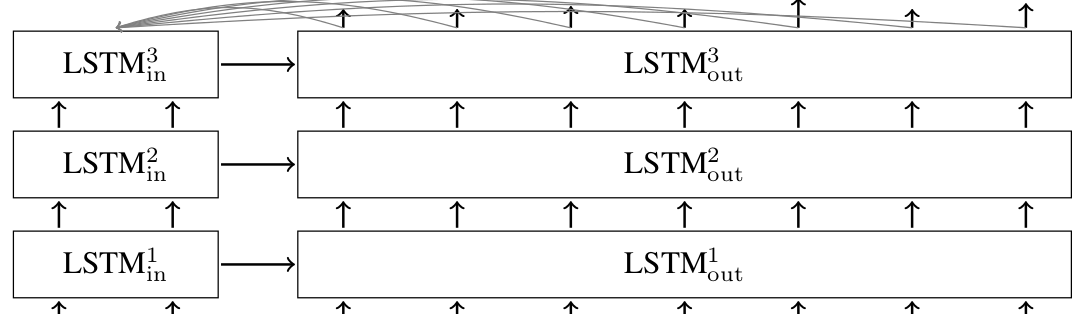
\includegraphics[width=0.7\textwidth]{pics/deep_seq2seq.png}
	\caption{A 3 layer Sequence-to-sequence model \cite{deep_seq2seq}. The lines pointing from the last decoder states to the last encoder represent an attention mechanism about which I talk in Section~\ref{sssec:311}}
\end{figure}

\subsubsection{Decoding and OOV}
In order to get the actual generated output sequences there are several techniques to decode from the probabilities of the words. One such technique is the Roulette Wheel selection, which is commonly used for genetic algorithms \cite{GA:1998}. Using this method at each time-step each word from the vocabulary can be generated with the probability computed from the softmax function. This is useful if we want to have some stochasticity in the decoding process, because it can produce slightly different outputs for the same source sequence. However it doesn't perform as well as the more frequent method used, which is to simply output the word with the highest probability from the softmax function. This is a greedy and deterministic approach since we will always get the same output for the same input.

While decoding a word at each time-step is fine a better approach is to the decode the whole output sequence at the same time, by outputting the sequence with the highest probability.
\begin{equation} \label{eq233}
\hat{T}=\arg\max_{T}p(T|S)
\end{equation}
Since in order to get the sequence with the highest probability we have to first generate all of the possible sequences a simple left-to-right beam search is usually employed to make the computation tractable. First, \(K\) words with the highest probability are retained in the first time-step, then at each time-step we expand this list by computing the joint probability of the partial sequences in the list and the words in the current time-step and retaining the \(K\) most probable partial sequences until we get to the end of the output sequence.

Another important aspect of sequence to sequence models applied to tasks involving language is the vocabulary.

\subsubsection{Bucketing and Padding}

\newpage\section{Background} \label{sec:background}
\subsection{Recent Chatbot Architectures and Augmentations} \label{ssec:31}
\subsubsection{Attention} \label{sssec:311}
\subsubsection{Context} \label{sssec:312}
\subsubsection{Objective Functions}
\subsubsection{Additional Features}
\subsubsection{Knowledge Bases, Copying and Information Retrieval}
\subsubsection{Task-Oriented Approaches}
\subsubsection{Decoding and Beam Search}
\subsubsection{Reinforcement Learning}
\subsubsection{Pretraining}
\subsubsection{Additional Encoder-Decoder Models}
\subsubsection{Evaluation Methods}

\subsection{Criticism} \label{ssec:32}
\subsubsection{Datasets}
\subsubsection{Loss Function}
\subsubsection{Memory}
\subsubsection{Evaluation Metrics}
\subsection{Summary} \label{ssec:33}
    

\newpage\section{Experiments} \label{sec:experiments}

\subsection{The Tranformer Model} \label{ssec:41}

\subsection{Datasets} \label{ssec:42}

\subsection{Training Details} \label{ssec:43}

\newpage\section{Results} \label{sec:results}
\subsection{Quantitative Analysis} \label{ssec:51}
\subsection{Qualitative Analysis} \label{ssec:52}

\newpage\section{Future Work} \label{sec:future}
\subsection{Ideas Towards Solving The Loss Function Issue} \label{ssec:61}
\subsection{Temporal Conditioning and Memory} \label{ssec:62}
\subsection{Additional Ideas} \label{ssec:63}

\newpage\section{Conclusion} \label{sec:conclusion}



\bibliographystyle{apalike}
\newpage\bibliography{chatbots}
\end{document}
